\section{Entorno de ejecución}
\subsection{LAM}
\url{http://www.dcs.ed.ac.uk/home/trollius/www.osc.edu/Lam/lam/tutorial.html}
\subsection{MPICH}
\url{https://www.dartmouth.edu/~rc/classes/intro_mpi/running_mpich2_ex.html}
\subsubsection{Instalación}



\subsubsection{Ejecución}

\begin{enumerate}
    \item Crear archivo llamado mpd.hosts que contendrá los nombres de las computadoras y el número de procesos en cada computadora donde ejecutará su programa.
\lstset{language=bash, breaklines=true, basicstyle=\footnotesize}
%\lstset{numbers=left, numberstyle=\tiny, stepnumber=1, numbersep=-7pt}
\begin{lstlisting}[frame=single] 
    slave1:4
    slave2:4
\end{lstlisting}



\lstset{language=bash, breaklines=true, basicstyle=\footnotesize}
%\lstset{numbers=left, numberstyle=\tiny, stepnumber=1, numbersep=-7pt}
\begin{lstlisting}[frame=single] 
    mpdboot -f mpd.hosts -n 2
    #note: 2 is the number of nodes you will be using
    mpiexec -np 8 mpi_program_name [program arguments]
    mpdallexit
\end{lstlisting}

\end{enumerate}


\begin{figure}[H]
    \centering
  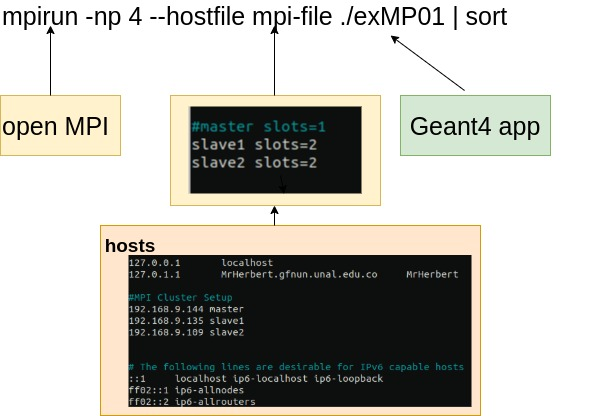
\includegraphics[width=0.7\textwidth]{images/execution.jpg}
  \caption{Esquema}
  \label{esq}
\end{figure}

\newpage